\chapter{Introduction}
\label{ch:introduction}

%% The following annotation is customary for chapter which have already been
%% published as a paper.

%% It is only necessary to list the authors if multiple people contributed
%% significantly to the chapter.
Humanity has long harnessed the power of wind for various applications ranging from simple sailing boats to grain mills and water pumps. Some researchers estimate wind energy has been in use for over 2000 years~\cite{kaldellis2011wind}. In the present day, wind energy is poised to play an important role in moving away from fossil fuel based sources of energy.

\section{Historical overview}
Beurskens~\cite{beurskens2014history} broadly classifies four different periods in which the use of wind energy evolved into its current form. 
\begin{enumerate}
\item 600–1890 (classical period) - Classic windmills mainly used as mechanical drives to operate grain mills and other applications. More than $100,000$ windmills were constructed in northwestern Europe. This period ended after the discovery of the steam engine and because of the ready availability of wood and coal. 
\item 1890–1930 - Development of the first electricity generating wind turbines. The development of electricity as a source of energy available to everyone led to the use of windmills as an additional possibility for generating electricity. This period saw some basic developments in the field of aerodynamics and control. This period ended as cheaper fossil fuels like oil became more readily available to generate electricity.
\item 1930–1973 - First phase of modern innovation. The necessity of electrifying rural areas and the shortage of energy during the Second World War stimulated new developments. This period saw major advances in the field of aerodynamics. 
\item From 1973 to present day - Second phase of innovation and mass production of wind turbines. The energy crisis and environmental problems in combination with technological advances ensure a commercial breakthrough.
\end{enumerate}

The classical wind turbines converted the kinetic energy of wind to mechanical energy directly and were likely vertical. The blades consisted of sailcloth and no control mechanisms were present. Yaw mechanisms were the first piece of technology adopted to align the turbines with the wind direction. Textile strips attached on the wooden blades and the pressure difference across the two sides of the blade kept the strips in place giving an aerodynamic profile. John Smeaton was one of the earliest pioneers in experimenting with aerodynamic efficiency of wind turbines. He introduced the twist in blades (which he termed as “weather”). More improvements to the technology steadily improved the performance of wind turbines but they were superseded by steam power after the invention of steam engines.

In the late 1800s, the rise in popularity of the dynamo reignited interest in using wind power to generate electricity and the earliest wind turbines generated a few kW of power. Development of wind turbines continued in Europe spurred largely by the unpredictability of oil prices during the early $20^{th}$ century. Denmark, US and Germany were the main hubs of innovations in wind energy in this period. The Smidth Company of Denmark introduced two blade turbines capable of producing 50kW and 70kW. A three bladed 200kW machine was installed in Gedser around the year 1957 (see for example figure~\ref{fig:windturbex1}). After the second world war, wind power saw gradual improvement in other areas spurred largely by increasing demand for electricity and reluctance to rely on fossil fuels for all power. The aerodynamic knowledge gained in the aerospace sector also played a key role. However, the progress started to slow as fossil fuels became cheaper and nuclear power emerged as a viable source of energy. And just as steam power had sidelined wind power almost a century earlier, nuclear energy and fossil fuels seemed to do the same until the oil crisis of 1973. 

A new energy policy was pursued after the oil crisis to address the over dependence on oil and also to account for the fact that fossil fuels could be exhausted if over used. Environmental problems with the use of fossil fuels and the danger of nuclear energy came to light almost a decade later. Once again, renewable sources of energy like wind, solar and geothermal were actively pursued. It was quickly realized that the only way for wind power to be economical was with large multi megawatt turbines. This phase of development saw large leaps in research in wind turbine design and associated fields like grid connections, wake flows, structures, installation among others. Offshore wind energy was identified as the best candidate for large wind farms. The first offshore farm was erected 2.5 km from the coast of Vindeby in Denmark in 1991 with a total capacity of 4.95 MW comprising 11 450kW turbines. 
More information about the history of wind turbines can be found in History of Wind by Buerskens~\cite{beurskens2014history}. 
\begin{figure}[h!]
    \centering
    \captionsetup{justification=centering}
    \begin{subfigure}[b]{0.45\textwidth}
    \centering
    \captionsetup{justification=centering}
        \includegraphics[width=0.75\textwidth]{ch1_introduction/images/postwindmill.png}
        \caption{A post wind mill in the Netherlands.}
    \end{subfigure}
    ~ %add desired spacing between images, e. g. ~, \quad, \qquad, \hfill etc. 
      %(or a blank line to force the subfigure onto a new line)
    \begin{subfigure}[b]{0.45\textwidth}
    \captionsetup{justification=centering}
        \includegraphics[trim=0 0 0 0,clip,width=0.9\textwidth]{ch1_introduction/images/Smidth-Aeromotor_fig120hist.png}
        \caption{Smidth-Aeromotor in Denmark.}
    \end{subfigure}
    \caption{Wind mills used for mechanical drives (a) and an out of service Smidth-Aeromotor in Denmark with a nominal output of $70kW$ (b)~\cite{beurskens2014history}.}
    \label{fig:windturbex1}
\end{figure}
\begin{figure}[h!]
    \centering
    \captionsetup{justification=centering}
 \begin{subfigure}[b]{0.45\textwidth}
 \centering
    \captionsetup{justification=centering}
        \includegraphics[trim=0 0 0 0,clip,width=0.45\textwidth]{ch1_introduction/images/petten_25mhawt.png}
        \caption{The $25 m$ HAT wind turbine in operation at Petten ($0.4 MW$ rated capacity)~\cite{beurskens2014history}.}
    \end{subfigure}
    \begin{subfigure}[b]{0.45\textwidth}
    \centering
    \captionsetup{justification=centering}
        \includegraphics[width=0.9\textwidth]{ch1_introduction/images/gehaliadex.jpg}
        \caption{The $12 MW$ GE Haliade X at the port of Rotterdam~\cite{GE}.}
    \end{subfigure}
    \caption{Evolution of wind turbines, from producing $<1 MW$ in 1980s (a) to large wind turbines producing $>10 MW$ today (b).}
    \label{fig:windturbex2}
\end{figure}

\section{Wind energy in the current energy climate}
While a period of steady but unspectacular growth in wind energy was observed in the early 1990s, in recent times it has grown spectacularly (figure~\ref{fig:wind_inst_hist}). Wind energy is expected to play a crucial role in transitioning towards a zero carbon energy sector. 
\begin{figure}[h!]
\centering
\captionsetup{justification=centering}
 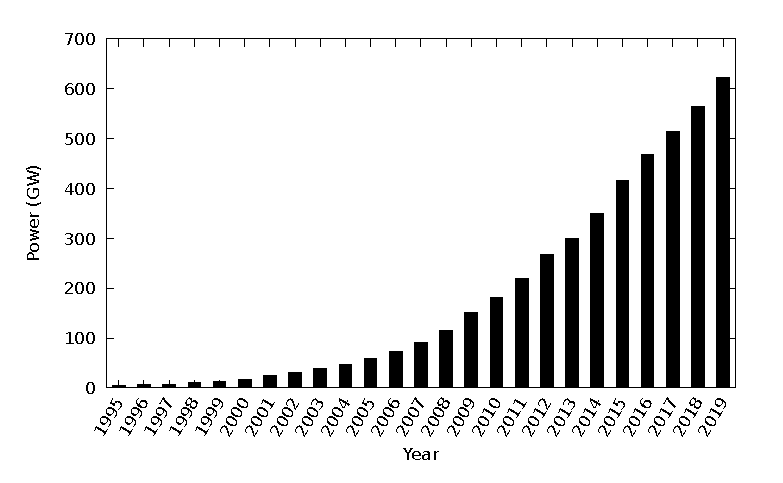
\includegraphics[width=0.85\textwidth]{ch1_introduction/images/wind_inst_cap_hist.eps}
\caption{Worldwide cumulative installed capacity of wind energy over time.}
 \label{fig:wind_inst_hist}
\end{figure} 
Constant improvements in wind turbine design has led to larger and larger wind turbines (figure~\ref{fig:wind_rotor}). Larger wind turbines (see figure~\ref{fig:windturbex2}) have driven installation costs per megawatt (MW) down which is reflected in the massive cost reduction for both onshore and offshore wind turbines. The global weighted-average levelized cost of energy (LCOE) of projects  using this technology and commissioned in 2019 was USD 0.053/kWh — $9\%$ lower than in 2018 and $39\%$ lower than in 2010, when it was USD 0.086/kWh. Onshore wind energy now consistently outcompetes even the cheapest fossil fuel fired source of electricity, while costs continue to decrease~\cite{irenareport}. 
\begin{figure}[h!]
\centering
\captionsetup{justification=centering}
 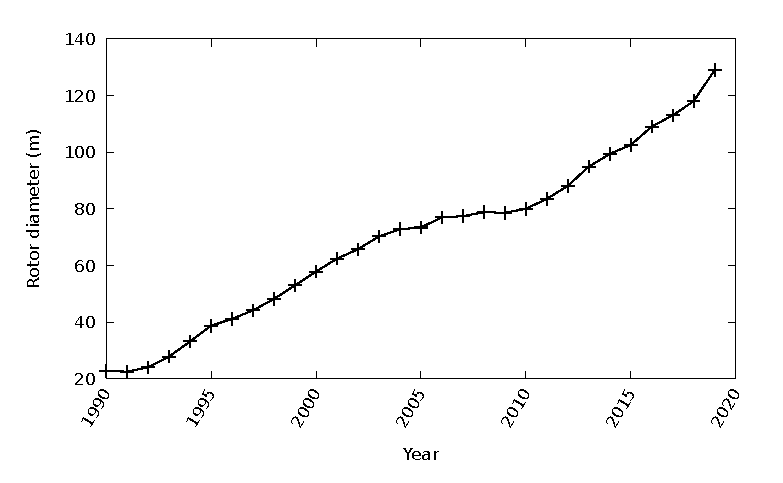
\includegraphics[width=0.85\textwidth]{ch1_introduction/images/wind_rotor_size.eps}
\caption{Rotor diameter size over years~\cite{rotorsize}.}
 \label{fig:wind_rotor}
\end{figure} 

Research on wind turbine aerodynamics have played a huge role in improving the performance of turbine blades over the years. Aerodynamicists have a variety of tools at their disposal. Over the years field experiments, wind tunnel measurements and computational tools have all been used to push the envelope of wind turbine aerodynamics. Looking ahead, the wind turbines are likely to become increasingly efficient and complex. To facilitate tackling the upcoming challenges, the tools used for research must also improve. Uncertainties in research tools must be reduced by using higher fidelity tools to keep up with the growth of technology. 

\section{Wind turbine aerodynamics}

Wind turbines operate at high Reynolds numbers and low Mach numbers which is somewhat unique compared to other external aerodynamic applications like aerospace, and greatly advantageous in terms of numerical analysis. The high Reynolds number means large regions of the flow can be considered inviscid except for a small region around the body known as the boundary layer (figure~\ref{fig:zonal}). The low Mach numbers imply that the flow remains incompressible. This combination of conditions have been exploited to develop a wide variety of numerical tools based on simplified forms of the Navier-Stokes equations.
\begin{figure}[h!]
\centering
\captionsetup{justification=centering}
 \includegraphics[width=0.5\textwidth]{ch1_introduction/images/zonal.png}
\caption{Inviscid flow and boundary layer regions~\cite{katz_plotkin_2001} for the flow around a wind turbine blade.}
 \label{fig:zonal}
\end{figure} 
On the other hand, aerodynamic analysis of wind turbines remains very challenging because of the disparate range of the scales involved (figure~\ref{fig:scales}). The relevant length scales range from boundary layers on the turbine blades that  are a few millimeters thick all the way upto wind farms that are tens of kilometers long. 
\begin{figure}[h!]
\centering
\captionsetup{justification=centering}
 \includegraphics[width=0.75\textwidth]{ch1_introduction/images/scales_porteagel.png}
\caption{Range of scales of flow that are relevant in wind turbine aerodynamics~\cite{porte2020wind}.}
 \label{fig:scales}
\end{figure} 

In the following sections, a review of wind turbine aerodynamics is presented in three parts - aerodynamics of airfoils, aerodynamics of rotors and wind farm analysis.

\subsection{Airfoil analysis}\label{ssec:ch1airfoil}
Airfoil aerodynamics is at the heart of wind turbine rotor aerodynamics. Two dimensional analysis of airfoils is required by many different rotor design methods. Also analyzing the flow over a simpler two dimensional airfoil can give much needed insight into the physics of wind turbine aerodynamics under complex flow conditions. Due to wind turbines operating at very high Reynolds numbers, the flow around airfoils can be divided into the boundary layer very near the airfoil surface and an inviscid region away from the surface. While the boundary layer region is crucial in many applications, the inviscid analysis can also give useful information especially in attached flow regions. By neglecting the effect of viscosity and assuming the flow to be irrotational, potential flow analysis can be used. Panel methods~\cite{katz_plotkin_2001} are very popular for the inviscid analysis of airfoils. The boundary layer can be analyzed separately by solving the simplified boundary layer equations~\cite{Lyon2014}. Integral boundary layer methods can further simplify the two dimensional boundary layer equations into a one dimensional problem. Combination of the boundary layer methods with potential flow methods can give the global flow field. This is known as the interacting boundary layer approach~\cite{Ozdemir2020} which is used in tools like XFOIL~\cite{drela1989xfoil} and RFOIL~\cite{rfoil_orig}.

However, the simplified analysis methods are only valid under attached flow conditions. While inviscid flow methods cannot be used to analyze separated flow, even boundary layer methods loose accuracy under such conditions. Passive flow control devices like vortex generators are widely used to improve the performance of the airfoil and delay separation. Potential flow methods and boundary layer methods cannot be used for such complex geometries readily. With increasing use of wind turbines in adverse weather conditions, rotor blades are also subject to erosion. Modeling such effects are also not yet possible with lower fidelity tools. 
\begin{figure}[h!]
\centering
\captionsetup{justification=centering}
 \includegraphics[width=0.5\textwidth]{ch1_introduction/images/airfoil_picture.png}
\caption{Velocity contours for a flow past an airfoil.}
 \label{fig:airfoil}
\end{figure} 

Computational Fluid Dynamics (CFD) methods do not have such limitations as the incompressible Navier Stokes equations are solved without any of the simplifying assumptions used for the methods mentioned above. Reynolds Averaged Navier Stokes (RANS) based methods are more widely used in combination with turbulence modeling, but the use of Large Eddy Simulations (LES), and hybrid LES methods are gaining traction. Some of the challenges for CFD in airfoil aerodynamics are the prediction of laminar to turbulent transition and flow separation.



\subsection{Rotor modeling}
%Blade aerodynamics - BEM, lifting line, Panel methods, CFD RANS, CFD DES (LES) ..
The design of rotor blades is a multi-disciplinary endeavour including aerodynamic analysis and structural design. Focusing on the aerodynamics only, due to faster computational times the Blade Element Momentum (BEM) theory is widely used in the early stages of the design process. The rotor design from BEM is then evaluated by an aeroelastic tool and if the design turns out to be efficient, it is evaluated by more advanced and accurate methods~\cite{bak2011aerodynamic} like CFD. The rotor design is carried out with the intention of maximizing Annual Enegy Production (AEP) which is traditionally done by a mixture of designer experience and numerical optimization. Due to this iterative nature of the design process, computational speed at a reasonable accuracy overrides other criteria for selecting numerical tools. 

BEM theory is the oldest method~\cite{windenergyexp, bak2011aerodynamic} that has been constantly improved over the years~\cite{Gerardthesis}. The local blade element theory is used in combination with the one dimensional momentum theory. The assumptions are that the flow is inviscid and there are no losses. The rotor plane is assumed to be an ideal and permeable disc that extracts energy~\cite{windenergyexp, bak2011aerodynamic}. Design of rotor blades is done iteratively based on two dimensional airfoil characteristics which can be found using the methods described in section~\ref{ssec:ch1airfoil} .

Vortex wake methods are a more accurate representation of the flow field around rotors. The flow is still assumed to be steady, but the rotor geometry is represented either as a lifting line~\cite{awsm_arne} or a lifting surface~\cite{katz_plotkin_2001}. Trailing and shed vortices are computed based on local flow conditions and airfoil characteristics. These vortices are then convected into the wake. In a lifting line model, the blade is represented by a single line with bound vorticity that varies radially. For lifting surfaces, the blade is represented by a zero thickness surface along the camber line instead of assuming that all lift is concentrated along a line, as is done in the lifting line theory. Three dimensional panel methods represent the exact geometry of the blade and are also used for rotor analysis. Similar to the two dimensional scenario, a potential flow solution is sought~\cite{katz_plotkin_2001, arne_phd}.
All the methods described so far are inviscid and as the fidelity of the representation of rotor increases from the lifting line to lifting surface and finally to the panel method, so does the computational requirements. 

CFD has also been used for rotor blade analysis. The first RANS simulations on wind turbine rotors were performed in the late 1990s and early 2000s~\cite{duque2000numerical, sorensen1998rotor, varela1999cfd}. A detailed historical overview of the use of CFD in rotor modeling can be found in Sumner et al~\cite{sumner2010cfd}. While the use of RANS turbulence models is still common, there have been some hybrid LES studies on rotors reported recently~\cite{criticalreview}. 

The inviscid methods rely to some extent on two dimensional airfoil characteristics and are prone to missing some three dimensional phenomena like rotational augmentation where it is observed that the inboard sections of blades produce lift and drag that is significantly different from the two dimensional characteristics~\cite{sumner2010cfd, schreck2002rotational}. Performing full three dimensional CFD analysis of rotors overcomes this limitation but that comes with an increase in computational cost. Some authors~\cite{xu2002development, schmitz2005parallelized} have proposed the use of a hybrid between CFD and inviscid vortex based methods. The region close to the rotor is modeled using CFD and the flow outside is modeled as inviscid using the inviscid methods described earlier. Hybrid approaches are especially useful in studying wake aerodynamics. 
\begin{figure}[h!]
\centering
\captionsetup{justification=centering}
\includegraphics[width=\textwidth]{ch1_introduction/images/turbine_wake_picture2.png}
\caption{Vortex structures behind a turbine blade (periodic CFD simulation).}
 \label{fig:rotor}
\end{figure} 

Another alternative to modeling rotor blades in CFD is the use of an actuator disc (AD)~\cite{aagaard1982actuator, rajagopalan1985finite}. The AD method is based on the blade element theory and represents the rotor with an equivalent porous surface and it is modeled as a source term that acts on the flow in that region. However, this method is mostly used to model wind farms to study the behavior of wakes which is the subject of the next section.

\subsection{Wind farms} 
The wakes emanating from wind turbines are unsteady and highly turbulent. In addition, these wakes also interact with the atmospheric boundary layer which is also dynamic and turbulent. Also wind turbines, especially offshore turbines, are clustered in large wind farms to reduce installation and maintenance costs. Because of the relatively close spacing however, the wake from the turbines interact with each other in addition to the atmospheric boundary layer. Turbines that are downstream of another turbine can see power losses in the range of $40\%$ in full wake conditions and experience increased fatigue loads~\cite{porte2020wind, stevensreview, sandresereview}.

The wind turbine wake can be divided into two regions~\cite{vermeer2003wind} - the near wake region that extends about $2$-$4$ rotor diameters downstream from the turbine and the far wake which is further downstream (see figure~\ref{fig:ablwake}). The near wake region is influenced greatly by wind turbine features like blade profile, nacelle and is highly complex and three dimensional. The far wake region, however, is influenced more by wind turbine parameters such as thrust and power coefficients, incoming flow etc. As the spacing between any two turbines in a wind farm is larger than the near wake, modeling the far wake accurately is more important than the near wake for understanding wind farm aerodynamics.
\begin{figure}[h!]
\centering
\captionsetup{justification=centering}
\includegraphics[width=0.75\textwidth]{ch1_introduction/images/wake_regions.png}
\caption{Schematic figure from Port{\'e}-Agel et al.~\cite{porte2020wind} showing the time averaged flow features resulting from the interaction of a wind turbine with the incoming turbulent (atmospheric) boundary layer.}
 \label{fig:ablwake}
\end{figure} 


Numerical modeling of wakes is done either using analytical models or the use of three dimensional CFD analysis where the rotors are represented as an actuator disc or line or surface~\cite{sorensonal, sandresereview}. Analytical models are used to predict the velocity deficit caused by the wind turbine wakes. These models have a lower accuracy compared to full 3D CFD simulations but have a very low computational cost. Analytical models mostly aim to predict the mean velocity deficit and do not consider the turbulence properties in the wake that can be significantly different from the undisturbed flow field. Thus, they are commonly used for design purposes like optimization of the wind farm layout, control of wind farms and other multi-disciplinary simulations. RANS modeling of wind farms have been extensively studied. Steady state tools like RANS are not suitable for capturing important dynamic wake effects that can significantly affect wind turbine loading.
As computational resources have improved, the use of LES to study wind farm aerodynamics have become very common~\cite{stevensreview, criticalreview}.

Reviews of wind turbine wake aerodynamics can be found in literature (for example, Sanderse et al~\cite{sandresereview},  Port{\'e}-Agel et al.~\cite{porte2020wind}, Stevens and Meneveau~\cite{stevensreview}, Th{\'e} and Yu~\cite{criticalreview}).



%\section{Outlook}
%However as the size of the turbine blades has increased, issues like thick airfoils, transition modeling are becoming more important. Additionally, new concepts to improve the efficiency of the turbines (e.g. vortex generators) are becoming more common. While it is possible to extend the existing tools like RFOIL to account for some of the new problems\cite{Ramanujam2016, Ramanujam2017, doublewake} arising out of modern wind turbine blades, they are still limited in their scope of applicability. Thus, a higher fidelity general purpose tool like CFD becomes necessary.
\subsection*{Looking ahead}
From the preceding section it can be seen that despite the vast range of scales involved in wind turbine aerodynamics, CFD methods are regularly used in all cases. As wind turbines become more complex, the use of a higher fidelity tool like CFD will become more prevalent. Additionally, CFD tools are increasingly being used in multi disciplinary problems like fluid structure interaction~\cite{hsu2012fsi, wang2016fsi, airfoilfsi}, shape optimization~\cite{madsenshapeopt, dhertshapeopt}, uncertainty quantification~\cite{andresuq, hsiehuq}, aeroacoustics~\cite{luolesacoust, edisonacoust} to name a few. It must be noted that the references cited here are only a small selection of the state of the art. While industrial adoption of CFD for the full rotor design is likely far away in the future, CFD methods are increasingly being used earlier in the design process instead of just being used for evaluation purposes. 

\section{Goal}

The main aim of this thesis is to develop a new pressure based solver within the framework of the open source multi-physics suite SU2~\cite{SU22013}. The immediate goals are to use this solver for various wind turbine aerodynamics applications like rotor simulations, vortex generator modeling and improving lower fidelity tools. In the long term, the goal is to take advantage of the open source nature of SU2 to not only improve the solver for aerodynamic applications but also to use it as a base for multi disciplinary applications like fluid structure interaction, aeroacoustics and optimization. 

\section{Dissertation overview}
This thesis can be broadly divided into two parts - Chapters 2, 3 and 4 are devoted to the implementation details of the new pressure based solver in SU2 while chapters 5, 6 and 7 focus on different applications of CFD in wind energy. 

Chapter 2 describes the governing equations for incompressible flow and different methods to solve them. First a short overview of the incompressible Navier Stokes equations is presented. The finite volume method that is commonly used in CFD is described for a general scalar equation highlighting the various numerical aspects. Subsequently, the challenges when dealing with the incompressible flow equations and different methods to overcome them are described. Finally, an overview on turbulence modeling for incompressible flows is given.

Chapter 3 describes the implementation of the governing equations and solution methods outlined in chapter 2 into SU2. 

Chapter 4 presents some verification and validation results for the new solver. Verification of the accuracy of the solver is carried out against analytical solutions. Different test cases that replicate different conditions faced in wind turbine aerodynamics are chosen to validate the solver. 

Chapter 5 presents the first steps towards modeling vortex generators in integral boundary layer methods. First a conceptual overview of the effect of vortex generators (VGs) on turbulent boundary layers is presented. CFD simulations of VGs on flat plates is then used to introduce the modeling approach. 
%Finally, a preliminary VG model is applied to a flat plate integral boundary layer tool and the results are compared against CFD results.

Chapter 6 presents the effect of leading edge erosion using roughness models for eddy viscosity based RANS turbulence models. The performance of the roughness models is first validated against empirical formulations and experimental data for a flat plate and airfoils. Different methods to characterize roughness numerically are surveyed. Finally, the impact of roughness on turbulent boundary layers are studied and future research required to model roughness in integral boundary layers are presented. 

Chapter 7 will present preliminary results from the CFD analysis of the widely studied New Mexico rotor blade.

\bibliographystyle{dissertation}
\bibliography{ch1_introduction/ch1bib}


%\begin{figure}[h!]
%\centering
%\captionsetup{justification=centering}
% \includegraphics[width=0.65\textwidth]{ch1_introduction/images/BEM_rotor_plane.png}
%\caption{Flow through the wind turbine rotor plane for BEM analysis~\cite{zhangthesis}.}
% \label{fig:bemintro}
%\end{figure} 

%\begin{figure}[h]
%    \centering
%    \begin{subfigure}[b]{0.45\textwidth}
%    \centering
%    \captionsetup{justification=centering}
%        \includegraphics[width=.75\textwidth]{ch1_introduction/images/turbine_picture.png}
%        \caption{Vorticity contour for flow past a turbine blade.}
%    \end{subfigure}
    ~ %add desired spacing between images, e. g. ~, \quad, \qquad, \hfill etc. 
      %(or a blank line to force the subfigure onto a new line)
%    \begin{subfigure}[b]{0.45\textwidth}
%    \centering
%    \captionsetup{justification=centering}
%        \includegraphics[width=0.75\textwidth]{ch1_introduction/images/turbine_wake_picture.png}
%        \caption{Vorticity shed from the turbine blade (periodic simulation).}
%    \end{subfigure}
%    \label{fig:rotor}
%    \caption{Vorticity contour for flow past a turbine blade.}
%\end{figure}
